\section{Clases implementadas por mí}\label{CreateClass}

\setbeamercolor{block title}{bg=blue!50!black,fg=white}
\setbeamercolor{block body}{bg=blue!20,fg=white}

\begin{frame}
    \begin{columns}[t]
        \begin{column}{.5\textwidth}
          \tableofcontents[sections={1-2},currentsection]
        \end{column}
        \begin{column}{.5\textwidth}
          \tableofcontents[sections={3-4},currentsection]
        \end{column}
    \end{columns}
\end{frame}

\subsection{Document.cs}

\begin{frame}[fragile]{Document.cs}
  
  \textbf{Document.cs}\\
  Esta clase es implementada con el propósito de almacenar en 3 propiedades que esta contiene, el nombre, 
  la dirección y el contenido ya normalizado de cada documento \emph{txt} encontrado en la que llamaremos nuestra 
  base de datos.

 \begin{figure}[h]
    \center
    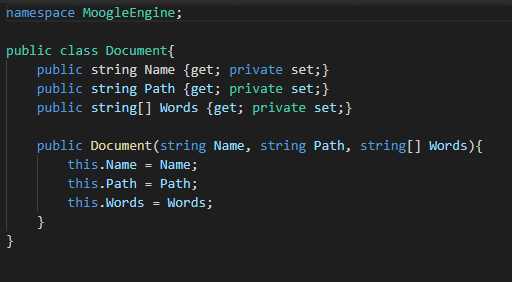
\includegraphics[width=5cm]{document.jpg}
    \caption{Código de la clase Document}
 \end{figure}

\end{frame}

\subsection{Operations.cs}

\begin{frame}[fragile]{Operations.cs}

  \only<1>{\textbf{Operations.cs}\\
  Objeto utilizado para realizar el pre-procesamiento de los datos encontrados en nuestra carpeta \textbf{"Content"},
  de forma que no sea necesario el procesamiento de todos estos datos cada vez que el usuario introduce una consulta.\\

  Este objeto utilizado en el proyecto bajo el nombre de \textbf{"dataBase"}, contiene un \emph{"vocabulary"} de extrema
  importancia para su correcto funcionamiento, ya que este diccionario se encarga de relacionar cada palabra que
  encontremos en nuestro corpus de documentos con la columna que le corresponderá en la matriz de TF-IDF.}


  \only<2>{El modelo de espacio vectorial \textbf{(TF-IDF)} permite representar los documentos con una estructura para poder realizar 
   tareas de filtrado, recuperación, indexación y calcular aquellas características o términos que aparecen en un
   documento.\\

   \begin{figure}[h]
    \center
    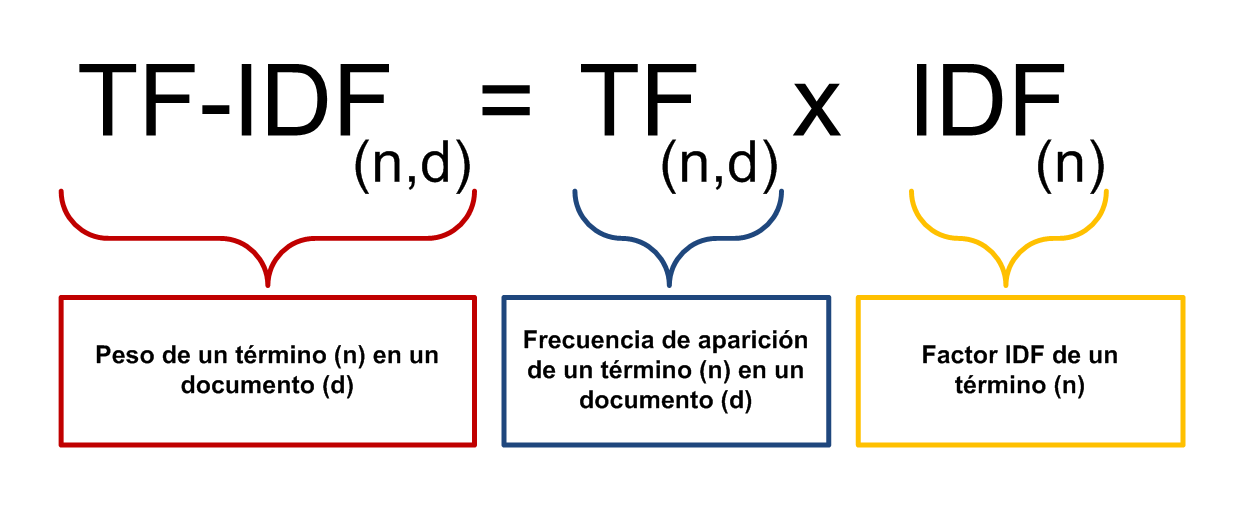
\includegraphics[width=6cm]{tfidf.jpg}
    \caption{Ponderación de la fórmula de TF-IDF}
   \end{figure}}

  \only<3>{A travéz de las fórmulas:\\

  \begin{equation}
    TF = \frac{n_d}{D}
  \end{equation} 

  Donde $n_d$ representa el número de veces que se repite una palabra en un documento y $D$ el número total de
  palabras que contiene ese documento.


  \begin{equation}
    IDF = \log(\frac{1+ N}{n_p})
  \end{equation} 

  Donde $N$ representa el número total de documentos y $n_p$ el número de documentos que contienen la palabra
  en cuestion.}
    
\end{frame}


\subsection{QueryOperations.cs}

\begin{frame}[fragile]{QueryOperations.cs}

  \only<1-2>{\textbf{QueryOperations.cs}\\
  Clase en la cual se desarrollan la mayoría de los métodos utilizados por el programa. De ellos los más notables son:}


  \only<2>{\textbf{Symbols:}\\
  Método que ayuda a determinar si el símbolo \$ se encuentra en una palabra y en caso de ser así, agrupa esta en una
  lista que será utilizada más adelante.\\
  El símbolo puede ser colocado en cualquier parte de la palabra, dándole mayor importancia a los documentos que la
  contengan, sólo el usuario debe asegurarse de que la palabra esté correctamente escrita.}

  \only<3>{\begin{figure}[h]
    \center
    \includegraphics[width=8cm]{Con \$.jpg}
    \caption{Búsqueda con \$}
 \end{figure}}

 \only<4>{\begin{figure}[h]
  \center
  \includegraphics[width=8cm]{Sin \$.jpg}
  \caption{Búsqueda sin \$}
 \end{figure}}


  \only<5>{\textbf{CosineSimilarity:}

  \begin{equation}
    \text{{CosineSimilarity}}=\frac{{A\cdot B}}{{\|Vert A \rVert \cdot \|Vert B \rVert}}   
  \end{equation}

 El objetivo de esta fórmula es calcular la similitud entre la pregunta (que se convertiría en el vector $A$,
 expresado en función de la aparición de los n términos en la expresión de búsqueda) y los m
 vectores de documentos almacenados, tomando $B$ momentaneamente como ellos.\\
 De tal forma que si el resultado es igual a 0, significa que los vectores son totalmente diferentes; y en caso
 de que sea igual a 1, son completamente iguales.}


  \only<6>{\textbf{Snippet:}
  
   \begin{figure}[h]
    \center
    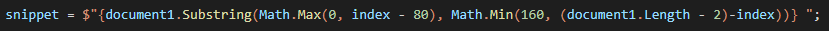
\includegraphics[width=10cm]{snippet.jpg}
    \caption{Función que se encarga de buscar un Snippet}
   \end{figure}
   
   Con esta simple función, que apartir de utilizar operaciones simples con son la \textbf{-} y la comparación
   de valores máximos y mínimos, extrae de un documento un fragmento de este donde casi siempre aparece la palabra
   en cuestion.}


  \only<7>{\textbf{LevenshteinDistance:}

  El algoritmo de Levenshtein utilizado para calcular la distancia entre dos cadenas de caracteres, utilizando
  la mínica cantidad de operaciones que incluyen la inserción, eliminación o sustitución de un caracter. \\

  Hace que su implementación usando \textbf{DP}(Programación Dinámica) de forma recursiva, conlleve crear una 
  matriz dp para almacenar los resultados de los subproblemas ya resueltos, y evitar el recálculo de estos. Esta 
  matriz tiene como dimensiones $[longitud\_de\_la\_cadena1 + 1, longitud\_de\_la\_cadena2 + 1]$.}
  
\end{frame}
 


